\documentclass[9pt,letterpaper]{extarticle}

\usepackage[left=0.5in,right=0.5in,top=0.58in,bottom=0.5in,headheight=11pt,headsep=6pt,footskip=14pt]{geometry}
\usepackage{amsmath}
\usepackage{booktabs}
\usepackage{array}
\usepackage{tabularx}
\usepackage{graphicx}
\usepackage{xcolor}
\usepackage{caption}
\usepackage{enumitem}
\usepackage{needspace}
\usepackage{fancyhdr}
\usepackage{lastpage}
\usepackage{microtype}
\usepackage{hyperref}

\graphicspath{{../figures/}}

\definecolor{navy}{RGB}{0,48,87}
\definecolor{slate}{RGB}{84,88,90}
\hypersetup{colorlinks=true, linkcolor=navy, urlcolor=navy,
  pdftitle={Corporate Default and Distress Prediction with Machine Learning}, pdfauthor={Thanh Vy Vo}}

\setlist{noitemsep, topsep=1pt, parsep=0pt, partopsep=0pt, leftmargin=13pt}
\setlength{\parskip}{2pt}
\emergencystretch=2em
\setlength{\parindent}{0pt}
\renewcommand{\arraystretch}{1.08}
\captionsetup{font=footnotesize, labelfont={bf,color=navy}, labelsep=period, skip=3pt, width=\textwidth}

\makeatletter
\renewcommand\section{\@startsection{section}{1}{\z@}{6pt plus 2pt minus 1pt}{3pt plus 1pt}%
  {\normalfont\large\bfseries\color{navy}}}
\renewcommand\subsection{\@startsection{subsection}{2}{\z@}{4pt plus 1pt minus 1pt}{2pt plus 1pt}%
  {\normalfont\normalsize\bfseries\color{navy}}}
\makeatother

\pagestyle{fancy}
\fancyhf{}
\lhead{\footnotesize\textcolor{slate}{\textbf{Corporate Default and Distress Prediction}}}
\rhead{\footnotesize\textcolor{slate}{\textbf{Thanh Vy Vo}}}
\lfoot{\footnotesize\textcolor{slate}{Data: anonymized firm-year panel, fiscal years 1999-2018}}
\rfoot{\footnotesize\textcolor{slate}{Page \thepage\ of \pageref{LastPage}}}
\renewcommand{\headrulewidth}{0.4pt}
\renewcommand{\footrulewidth}{0.4pt}

\begin{document}

% ======================================================================
% PAGE 1: summary, annual default-rate picture, data/design/definitions
% ======================================================================
\begin{center}
  {\Large\bfseries\color{navy} Corporate Default and Distress Prediction with Machine Learning}\\[2pt]
  {\normalsize Thanh Vy Vo}
\end{center}
\vspace{-4pt}

\section*{Summary}
\begin{itemize}
  \item Default is rare: 609 of 78,682 firm-years (0.77\%), so a rule that flags no firm is right for 99.0\% of test firm-years. The annual rate runs from 0.06\% (2000) to 1.50\% (2009); the early-2000s years average 0.23\%, below the overall rate, so this dataset shows no default spike there, while the Global Financial Crisis years average 1.40\%, above it.
  \item Settings were chosen on validation by ROC-AUC (LASSO C = 0.1, Ridge C = 0.01), and neither rebalancing treatment qualified under the pre-specified rule (selected: Unweighted). On test, LASSO (0.742), Ridge (0.738), the forest (0.734) and XGBoost (0.735) are similar on ROC-AUC under the resampling rule (all six pairwise differences similar; the LASSO--Ridge interval only just includes zero); Model 1 (0.721) is lower than LASSO and Ridge, and the decision tree (0.691) is lower than the forest and XGBoost.
  \item Ridge, the deployment model by the frozen validation rule, has a default rate of 3.74\% in its highest-risk test decile (3.86 times the test rate of 0.97\%), which holds 38.7\% of test defaults; at its validation threshold it flags 203 firm-years, of which only 16 default, and a fixed 0.50 cutoff flags no firm-year under any of the six models.
  \item Raw Ridge probabilities are too low (mean 0.57\% against 0.97\% observed on test). Platt scaling fitted on validation moves the mean to 0.93\% and gives a lower Brier score (0.00948 against 0.00954) without changing the ranking; isotonic regression is similar to raw on Brier under the resampling rule (the interval only just includes zero) and lower on PR-AUC.
  \item In stress periods (in-sample), the early-2000s rate of 0.23\% is below the other years' 0.78\% (no spike in this dataset) and the crisis rate of 1.40\% is above it; return and volatility shift most in both, and the market-only model separates defaulters less well than the accounting-only model in the crisis years. Recommendation: deploy Ridge with XGBoost as challenger (the pre-specified rule coincides with the highest validation ROC-AUC; no switch to the test leader, no complexity for a small, noisy margin).
\end{itemize}

\begin{center}
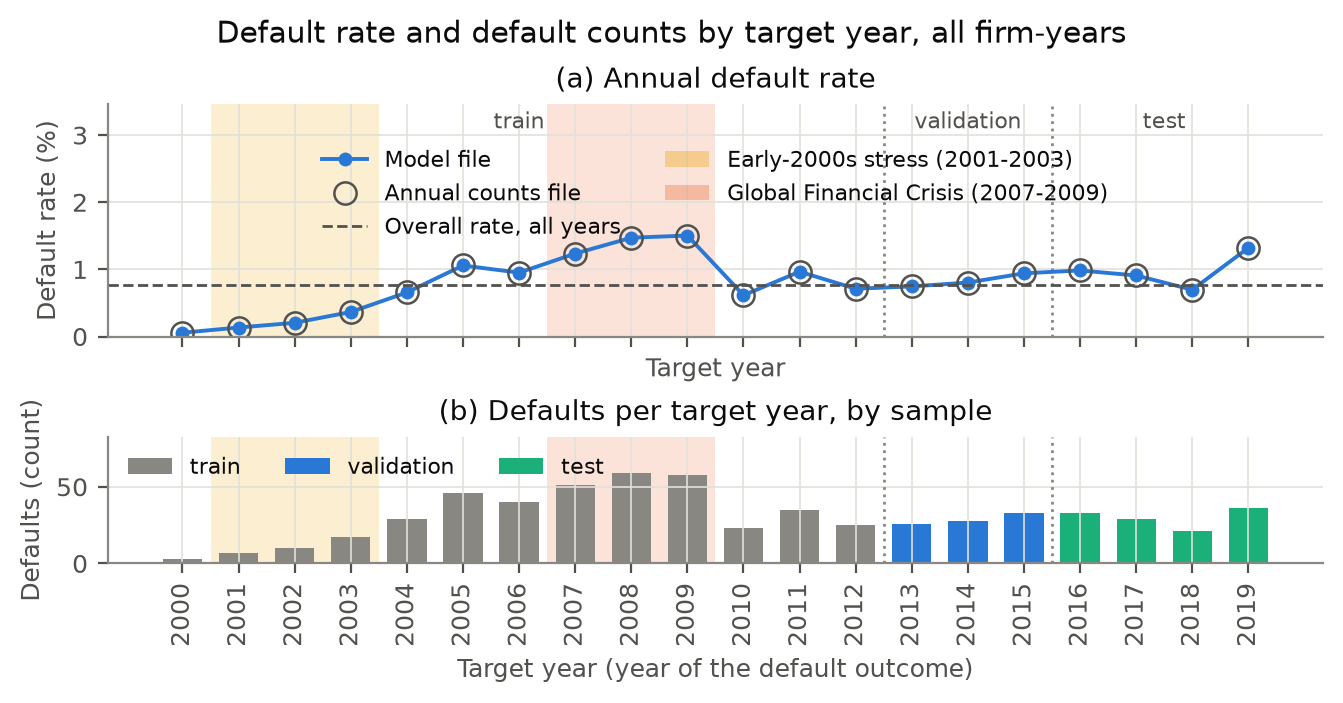
\includegraphics[width=0.68\textwidth]{annual_default_rate.png}
\par\vspace{1pt}
\captionof{figure}{Default outcomes by target year (2000--2019), all 78,682 firm-years (609 defaults). (a) Default rate in percent of firm-years; solid markers: model file, hollow markers: annual counts file; dashed line: overall rate. (b) Number of defaults. Shading marks the early-2000s stress (2001--2003) and the Global Financial Crisis (2007--2009); dotted lines separate the training, validation and test target years (aggregate counts only).}
\end{center}

\section*{Data, design and definitions }
{\small
\begin{itemize}
  \item \textbf{Data and split.} 78,682 firm-years of 8,262 firms, fiscal years 1999--2018, with 609 defaults (0.77\%). Predictors at fiscal year $t$ forecast default in year $t+1$. Chronological split, never shuffled: training fiscal years 1999--2011 (55,927 firm-years, 403 defaults, 0.72\%), validation 2012--2014 (10,473 firm-years, 87 defaults, 0.83\%), test 2015--2018 (12,282 firm-years, 119 defaults, 0.97\%).
  \item \textbf{Predictors and Model 1.} 21 continuous predictors (accounting ratios and market variables) in five groups (liquidity, leverage, profitability, efficiency, market) plus the industry category (10 levels, one-hot); standardization is fitted on training rows only. Models 2--6 use all of them; Model 1 (unpenalized logistic regression) omits Equity / assets and COGS / sales, which equal one minus Debt / assets and one minus Gross margin, because an unpenalized model with both members of a pair has no unique solution.
  \item \textbf{Selection and test lock.} Hyperparameters and the best model in each family are chosen by validation ROC-AUC (threshold-free, more stable than PR-AUC with few defaults); candidates within 0.0001 of the best count as equivalent and go to the smaller C, then the first in grid order, then the lower model number. Deployment rule: the best validation model is deployed if it is linear; a non-linear best model only if the best linear model is lower under the resampling rule (a linear model is preferred because it is transparent, auditable and adds no complexity for a small, noisy margin). Models are fitted on training firm-years only, with no refit. Test outcomes enter only Section 1's aggregate counts and data-integrity checks (one default per firm, raw/model agreement); none is used for any model, setting, threshold or calibration before the freeze, and no final model is fitted, tuned or selected after the unlock.
  \item \textbf{Class imbalance.} Class weighting and random 1:1 undersampling of training non-defaults are compared with unweighted fitting on Model 1's specification, on validation. A treatment is adopted only if its validation PR-AUC is higher than unweighted by the firm resampling check and its ROC-AUC is not lower; it then applies to Model 1 only. Only training data are rebalanced.
  \item \textbf{Thresholds, deciles, calibration.} Each model's classification threshold maximizes validation F1 (ties: highest threshold); a firm-year is flagged at or above it, applied unchanged to test. Deciles sort firm-years by predicted probability (ties broken by a fixed random key) into 10 equal groups: Decile 1 is the highest predicted risk. For the model with the strongest validation ROC-AUC, Platt scaling (two parameters, suited to few validation defaults; recorded as primary in the frozen choices before the test unlock) and isotonic regression are fitted on validation predictions only.
  \item \textbf{Resampling rule.} Comparisons resample whole firms with replacement (2,000 draws, shared across models); a model is called higher or lower only if the middle 95\% of the difference excludes zero, otherwise similar. The check is descriptive and ignores year-to-year (regime) uncertainty.
  \item \textbf{Metrics.} ROC-AUC; PR-AUC (average precision); KS = max(TPR $-$ FPR); precision, recall, F1 at the validation threshold; top-decile capture = share of defaults in Decile 1; Brier = mean squared probability error.
\end{itemize}
}

% ======================================================================
% PAGE 2: models and test comparison
% ======================================================================
\clearpage
\section*{Models and test comparison (Sections 2--5)}
\begin{center}
\footnotesize
\setlength{\tabcolsep}{2.4pt}
\begin{tabular}{@{}p{2.9in}*{9}{r}@{}}
\toprule
\textbf{Model (setting)} & \shortstack[r]{\textbf{Valid.}\\\textbf{ROC-AUC}} & \shortstack[r]{\textbf{Test}\\\textbf{ROC-AUC}} & \shortstack[r]{\textbf{Test}\\\textbf{PR-AUC}} & \shortstack[r]{\textbf{Test}\\\textbf{KS}} & \shortstack[r]{\textbf{Valid.}\\\textbf{threshold}} & \shortstack[r]{\textbf{Prec.}\\\textbf{(\%)}} & \shortstack[r]{\textbf{Recall}\\\textbf{(\%)}} & \textbf{F1} & \shortstack[r]{\textbf{Top-decile}\\\textbf{capture (\%)}} \\
\midrule
\textbf{M1 Logit} \scriptsize{(no penalty)} & 0.690 & 0.721 & 0.036 & 0.343 & 0.0203 & 6.5 & 10.9 & 0.082 & 36.1 \\
\textbf{M2 LASSO} \scriptsize{(C = 0.1)} & 0.696 & 0.742 & 0.048 & 0.407 & 0.0180 & 7.0 & 14.3 & 0.094 & 38.7 \\
\textbf{M3 Ridge}$^{\dagger}$ \scriptsize{(C = 0.01)} & 0.697 & 0.738 & 0.046 & 0.405 & 0.0183 & 7.9 & 13.4 & 0.099 & 38.7 \\
\textbf{M4 Tree} \scriptsize{(depth 4, min leaf 50)} & 0.632 & 0.691 & 0.020 & 0.317 & 0.0181 & 3.2 & 9.2 & 0.047 & 24.4$^{*}$ \\
\textbf{M5 Forest} \scriptsize{(200 trees, depth 6, min leaf 100, max features sqrt)} & 0.677 & 0.734 & 0.048 & 0.377 & 0.0176 & 7.9 & 10.1 & 0.089 & 35.3 \\
\textbf{M6 XGBoost} \scriptsize{(200 rounds, learning rate 0.03, depth 2)} & 0.682 & 0.735 & 0.038 & 0.382 & 0.0181 & 5.9 & 9.2 & 0.072 & 32.8 \\
\bottomrule
\end{tabular}
\par\vspace{1pt}\begin{minipage}{\textwidth}\raggedright\scriptsize Precision, recall, F1 and top-decile capture are test values (at the validation threshold); ROC-AUC, PR-AUC and KS are as labelled.\end{minipage}
\par\vspace{1pt}\begin{minipage}{\textwidth}\raggedright\scriptsize $^{\dagger}$ Deployment model by the frozen validation rule (Model 3: Ridge logistic (L2)); it is also the model with the strongest validation ROC-AUC.\end{minipage}
\par\vspace{1pt}\begin{minipage}{\textwidth}\raggedright\scriptsize $^{*}$ M4 Tree: top-decile capture depends on the random order of 2,504 tied firm-years (791 enter Decile 1); tie-averaged value 23.6\%.\end{minipage}
\par\vspace{2pt}
\captionof{table}{Final model comparison. Models are fitted on training firm-years (fiscal 1999--2011) with settings chosen on validation firm-years (fiscal 2012--2014, 10,473 firm-years, 87 defaults) and scored once on test firm-years (fiscal 2015--2018, target years 2016--2019: 12,282 firm-years of 3,712 firms, 119 defaults). Top-decile capture: percent of test defaults among the 10\% of test firm-years with the highest predicted probability.}
\end{center}

\begin{center}
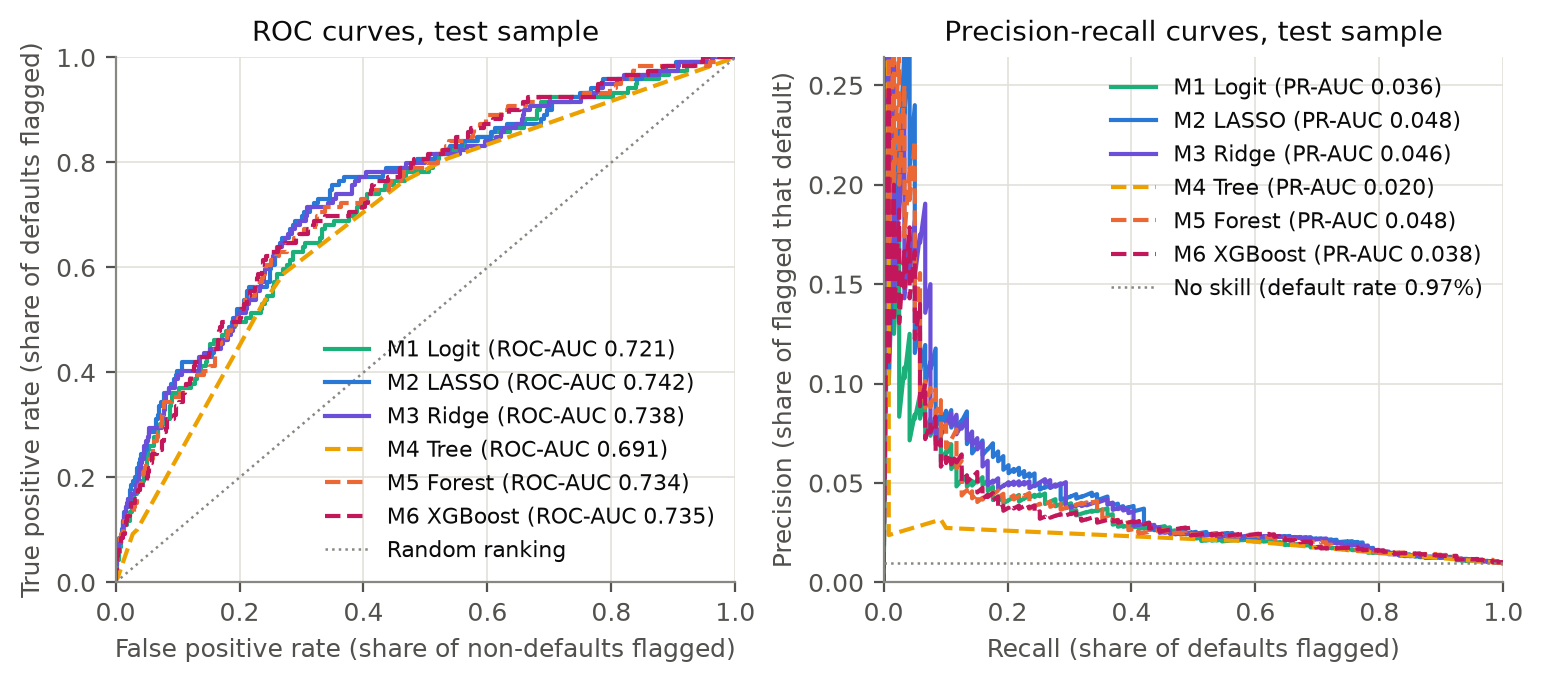
\includegraphics[width=0.78\textwidth]{roc_pr_test.png}
\par\vspace{1pt}
\captionof{figure}{Test firm-years, target years 2016--2019 (12,282 firm-years, 119 defaults). (a) ROC curves and (b) precision-recall curves of the six models; the dotted lines are random ranking and the test default rate (0.97\%). The precision axis is truncated, so precision at recall below 5\% is off-scale.}
\end{center}

\begin{itemize}
  \item \textbf{Regularization.} Selected by validation ROC-AUC, LASSO uses C = 0.1 and zeroes 18 of 31 coefficients (19 in an alternative solution with the same fit, since the split between Debt / assets and Equity / assets is arbitrary; given the other predictors the zeros add little predictive information and do not show a variable is unrelated to default, for example EBIT / assets is zero while EBITDA / assets is kept, r = +0.99); Ridge uses C = 0.01 (grid spanning only 0.691 to 0.697). The ten largest coefficients overlap in 7 (Models 1 and 2), 6 (1 and 3) and 8 (2 and 3) of 10 variables and the rank correlation of absolute coefficients with Model 1 is only 0.52 and 0.29, though the LASSO figures include that arbitrary split.
  \item \textbf{Single tree, forest, boosting.} On validation ROC-AUC the single tree (0.632) is lower than the forest (0.677; difference $-$0.045 [$-$0.072, $-$0.021]) and than XGBoost (0.682; $-$0.050 [$-$0.089, $-$0.012]), while the forest and XGBoost are similar ($-$0.005 [$-$0.029, +0.023]): these data do not show that boosting beats bagging. Both ensembles are similar to Ridge (Ridge minus forest +0.020 [$-$0.010, +0.050]; Ridge minus XGBoost +0.015 [$-$0.004, +0.034]), so the extra flexibility brings no detectable validation gain.
  \item \textbf{Test ranking.} Test ROC-AUC is 0.742 [0.696, 0.787] for LASSO, 0.738 for Ridge, 0.735 for XGBoost, 0.734 for the forest, 0.721 for Model 1 and 0.691 for the tree. The first four are similar under the resampling rule (all six pairwise differences similar; the LASSO--Ridge interval only just includes zero); Model 1 is lower than LASSO ($-$0.022 [$-$0.034, $-$0.010]) and Ridge ($-$0.018 [$-$0.027, $-$0.009]), and the tree is lower than the forest and XGBoost while LASSO and Ridge are higher than it. Test ROC-AUC exceeds validation ROC-AUC for every model (different samples, intervals overlapping).
  \item \textbf{Thresholds and imbalance.} Thresholds maximize validation F1; for Ridge, 203 test firm-years are flagged, 16 default and 187 do not (precision 7.9\%, recall 13.4\%), and precision is below 10\% for all six models; the right cut-off depends on the cost of a missed default against a false alarm. In Table 2, weighting leaves ranking unchanged within noise and undersampling has a lower ROC-AUC ($-$0.029 [$-$0.052, $-$0.005]) that depends on the draw (20 draws: 0.659 to 0.697, mean 0.677), and both move the 0.50 operating point: the unweighted fit flags none, the weighted and undersampled fits flag 2,127 and 2,493 validation firm-years.
\end{itemize}

\begin{center}
\footnotesize
\setlength{\tabcolsep}{3.2pt}
\begin{tabular}{@{}l*{10}{r}@{}}
\toprule
& & & & \multicolumn{3}{c}{\textbf{At the 0.50 cutoff}} & \multicolumn{4}{c}{\textbf{At own max-F1 threshold}} \\
\cmidrule(lr){5-7}\cmidrule(lr){8-11}
\textbf{Treatment} & \shortstack[r]{\textbf{ROC-}\\\textbf{AUC}} & \shortstack[r]{\textbf{PR-}\\\textbf{AUC}} & \shortstack[r]{\textbf{Top-decile}\\\textbf{capture (\%)}} & \shortstack[r]{\textbf{Flagged}\\\textbf{(count)}} & \shortstack[r]{\textbf{Prec.}\\\textbf{(\%)}} & \shortstack[r]{\textbf{Recall}\\\textbf{(\%)}} & \shortstack[r]{\textbf{Valid.}\\\textbf{threshold}} & \shortstack[r]{\textbf{Flagged}\\\textbf{(count)}} & \shortstack[r]{\textbf{Prec.}\\\textbf{(\%)}} & \shortstack[r]{\textbf{Recall}\\\textbf{(\%)}} \\
\midrule
\textbf{Unweighted}$^{\dagger}$ & 0.690 & 0.025 & 29.9 & 0 & n/a (none flagged) & 0.0 & 0.0203 & 105 & 6.7 & 8.0 \\
Class-weighted (balanced) & 0.687 & 0.025 & 31.0 & 2,127 & 1.8 & 44.8 & 0.7690 & 86 & 8.1 & 8.0 \\
Random undersampling (1:1) & 0.662 & 0.021 & 28.7 & 2,493 & 1.5 & 42.5 & 0.7599 & 183 & 6.0 & 12.6 \\
\bottomrule
\end{tabular}
\par\vspace{1pt}\begin{minipage}{\textwidth}\raggedright\scriptsize $^{\dagger}$ Treatment selected by the pre-specified validation rule and used for Model 1.\end{minipage}
\par\vspace{2pt}
\captionof{table}{Class-imbalance comparison on validation firm-years (fiscal 2012--2014, 10,473 firm-years, 87 defaults), Model 1 specification fitted on training firm-years (55,927 rows; 806 undersampled, all 403 defaults kept). Selected by the pre-specified rule: Unweighted. Max-F1 threshold: each treatment's own validation cutoff.}
\end{center}

% ======================================================================
% PAGE 3: risk deciles
% ======================================================================
\clearpage
\section*{Risk deciles (Section 5)}
\begin{center}
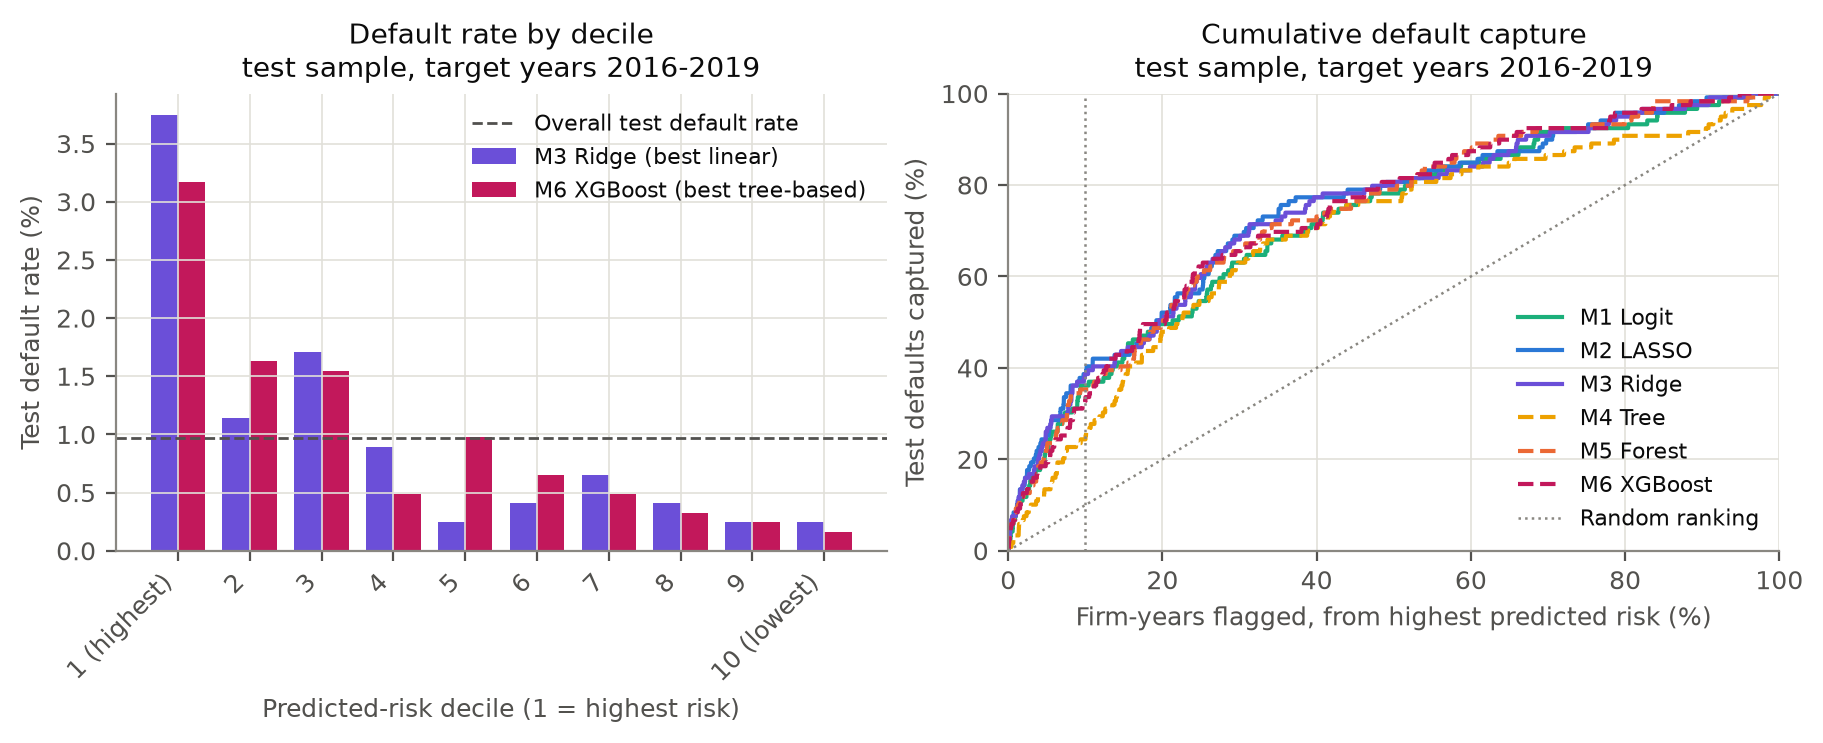
\includegraphics[width=0.92\textwidth]{risk_deciles_test.png}
\par\vspace{1pt}
\captionof{figure}{Test firm-years, target years 2016--2019 (12,282 firm-years, 119 defaults). (a) Default rate (\%) by predicted-risk decile for the linear model (M3 Ridge) and the tree-based model (M6 XGBoost) with the highest validation ROC-AUC in their family (Decile 1 = highest predicted risk; dashed line: test default rate). (b) Share of test defaults captured (\%) against the share of firm-years flagged from highest predicted risk, six models.}
\end{center}

\begin{center}
\footnotesize
\setlength{\tabcolsep}{5pt}
\begin{tabular}{@{}l*{6}{r}@{}}
\toprule
\shortstack[r]{\textbf{Predicted-risk}\\\textbf{decile}} & \shortstack[r]{\textbf{Firm-}\\\textbf{years}} & \shortstack[r]{\textbf{Distinct}\\\textbf{firms}} & \shortstack[r]{\textbf{Defaults}\\\textbf{(count)}} & \shortstack[r]{\textbf{Default}\\\textbf{rate (\%)}} & \shortstack[r]{\textbf{Share of all}\\\textbf{defaults (\%)}} & \shortstack[r]{\textbf{Cumulative}\\\textbf{capture (\%)}} \\
\midrule
1 (highest risk) & 1,229 & 621 & 46 & 3.74 & 38.7 & 38.7 \\
2 & 1,228 & 857 & 14 & 1.14 & 11.8 & 50.4 \\
3 & 1,228 & 926 & 21 & 1.71 & 17.6 & 68.1 \\
4 & 1,228 & 956 & 11 & 0.90 & 9.2 & 77.3 \\
5 & 1,228 & 983 & 3 & 0.24 & 2.5 & 79.8 \\
6 & 1,229 & 973 & 5 & 0.41 & 4.2 & 84.0 \\
7 & 1,228 & 962 & 8 & 0.65 & 6.7 & 90.8 \\
8 & 1,228 & 930 & 5 & 0.41 & 4.2 & 95.0 \\
9 & 1,228 & 857 & 3 & 0.24 & 2.5 & 97.5 \\
10 (lowest risk) & 1,228 & 638 & 3 & 0.24 & 2.5 & 100.0 \\
\midrule
\textbf{All test firm-years} & 12,282 & 3,712 & 119 & 0.97 & 100.0 & 100.0 \\
\bottomrule
\end{tabular}
\par\vspace{2pt}
\captionof{table}{Risk deciles of the deployment model (Model 3: Ridge logistic (L2)) on test firm-years, target years 2016--2019. Decile 1 (highest risk) holds the firm-years with the highest predicted probability; deciles differ in size by at most one firm-year. Firms: distinct firms in the decile. Cumulative capture: percent of all test defaults in Deciles 1 to the row's decile.}
\end{center}

\begin{itemize}
  \item \textbf{Deployment-model deciles (Table 3).} For Ridge, Decile 1 has a default rate of 3.74\% (lift 3.86) and holds 46 of the 119 test defaults (38.7\%); cumulative capture is 50.4\% after two deciles and 68.1\% after three. The pattern is not perfectly monotone (Decile 3 is above Decile 2). XGBoost, the tree-based model with the highest validation ROC-AUC, captures 32.8\%: Ridge minus XGBoost is +5.9 percentage points [$-$0.8, +12.2], similar. The decision tree is lower than Ridge (Ridge minus tree +14.3 percentage points [+3.8, +22.5]), but every comparison with its 24.4\% is sensitive to tie handling: it depends on the random order within a block of 2,504 firm-years sharing one predicted probability (791 enter Decile 1), and its tie-averaged value is 23.6\%.
  \item \textbf{Why the highest ROC-AUC need not have the highest PR-AUC.} On point estimates LASSO has both the highest test ROC-AUC (0.742) and the highest test PR-AUC (0.048), but its PR-AUC margin over the forest is negligible (LASSO minus forest +0.0001 [$-$0.025, +0.030], similar). The orders differ below the top (the forest is 4th on ROC-AUC but 2nd on PR-AUC, 0.048; Ridge is 2nd and 3rd), within noise (ROC-AUC +0.008 [$-$0.015, +0.030], similar), and the forest's reordering is specific to this seed. The general reason is that ROC-AUC averages over the whole ranking and is dominated by the many non-defaults, while PR-AUC mostly reflects the very top, where a few firm-years can reorder it.
  \item \textbf{Why a low misclassification rate can mislead.} Flagging no firm-year misclassifies exactly the defaults, a rate of 0.97\% on test, and at the 0.50 cutoff all six models flag 0 firm-years, with that same rate and recall of 0.0\%. The models whose thresholds do flag firm-years have a higher misclassification rate, from 2.00\% (forest) to 3.62\% (tree; Ridge 2.36\%), yet they are the ones that detect defaults (Ridge recall 13.4\%); minimizing misclassification would choose a model that finds nothing.
  \item \textbf{Why ranking is useful when the 0.50 cutoff fails.} At the 0.50 cutoff every model flags 0 test firm-years: the largest test probability is 0.070 (Model 1), 0.057 (LASSO), 0.053 (Ridge), 0.077 (tree), 0.028 (forest) and 0.048 (XGBoost), all far below 0.50. A general reason is that defaults are rare in the training years the models were fitted on (0.72\%). The ranking is still informative: every model captures more than 10\% of defaults in its top decile, from 24.4\% (tree; 23.6\% averaged over tie orders) to 38.7\% (LASSO), and Ridge's top decile has 25.72 non-defaults for every default captured, so reviewing that group costs false alarms.
  \item \textbf{Why similar AUC values can hide different decile behaviour.} In concept, AUC averages over the whole ranking while deciles weight specific regions, so similar averages can coexist with different behaviour in one region. Among the 9 model pairs with similar test ROC-AUC, a top-decile difference is detected in 1 pair: Model 1 against the tree (ROC-AUC difference +0.030 [$-$0.003, +0.062], similar; top-decile difference +11.8 percentage points [+1.7, +20.7], higher), and that pair is tie-sensitive (a block of 2,504 tied firm-years straddles the Decile 1 boundary; tie-averaged capture 23.6\%), so its ``higher'' label should be read with care. Decile rates beyond the top decile were not resampling-tested, so the data neither establish nor rule out the pattern for the other pairs.
\end{itemize}

% ======================================================================
% PAGE 4: calibration and interpretation
% ======================================================================
\clearpage
\section*{Calibration and interpretation (Section 6)}
\begin{center}
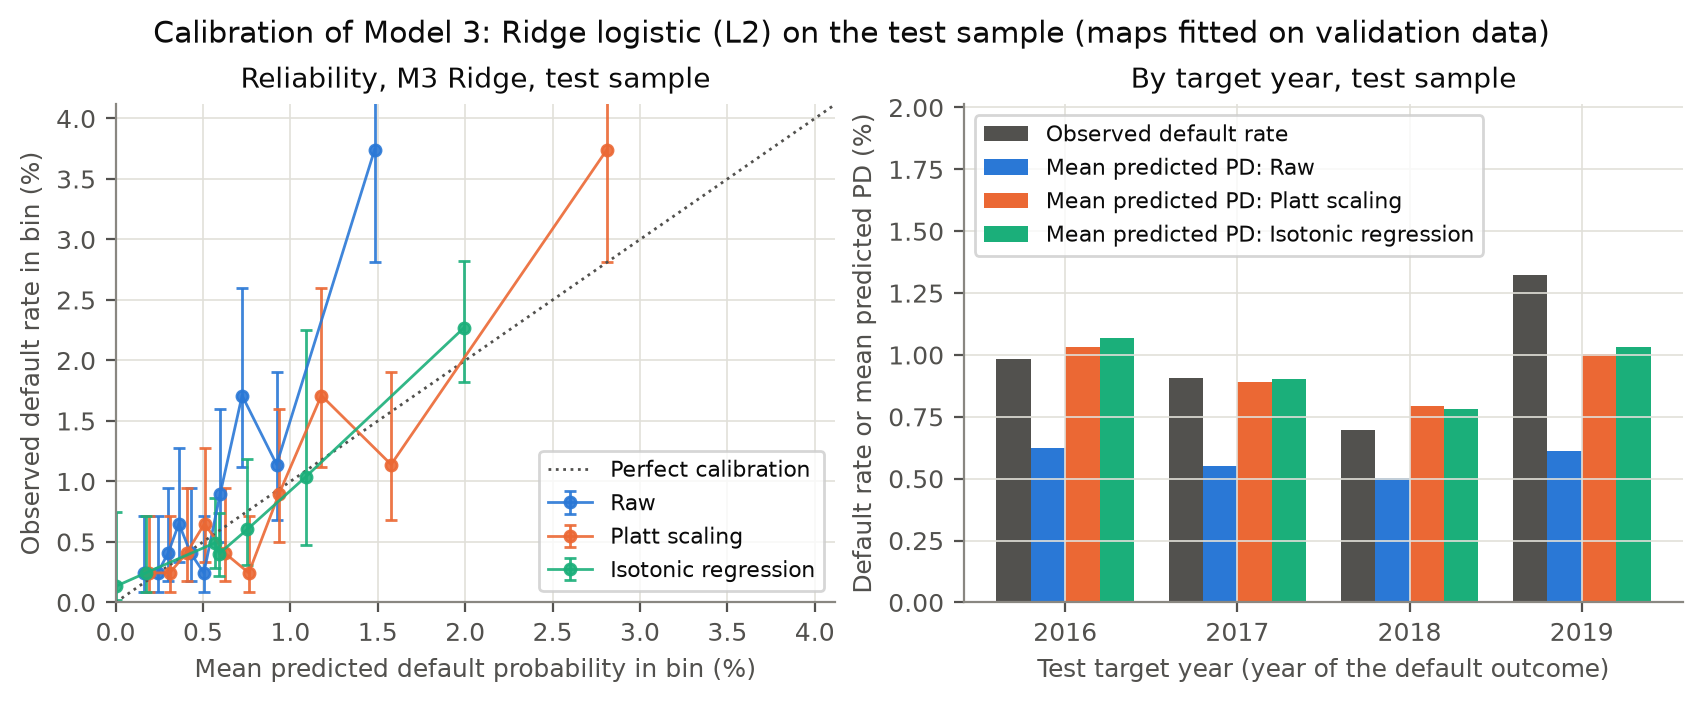
\includegraphics[width=0.86\textwidth]{calibration_test.png}
\par\vspace{1pt}
\captionof{figure}{Calibration of the model with the strongest validation ROC-AUC (Model 3: Ridge logistic (L2)) on test firm-years, target years 2016--2019 (12,282 firm-years, 119 defaults). (a) Mean predicted against observed default rate (\%) in ten quantile bins of each series' own probabilities (fewer, unequal for isotonic because of ties), raw and after validation-fitted Platt and isotonic maps; bars: 95\% Wilson intervals (top raw and Platt bars clipped). (b) Observed and mean predicted rate (\%) by test target year.}
\end{center}

\begin{center}
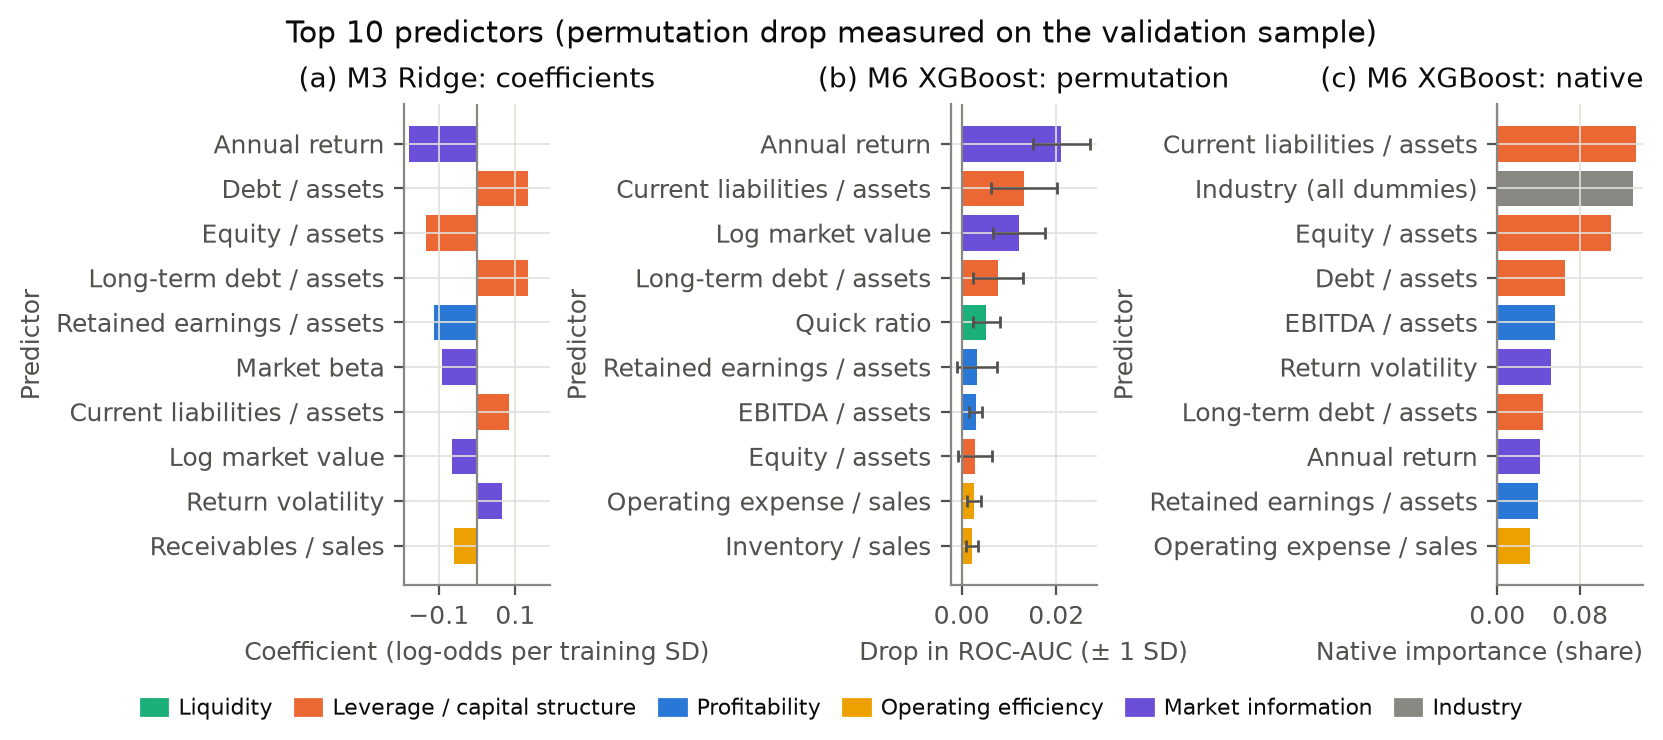
\includegraphics[width=0.84\textwidth]{importance_comparison.png}
\par\vspace{1pt}
\captionof{figure}{Most important predictors. (a) Standardized coefficients of the linear model selected by validation ROC-AUC (M3 Ridge). (b) Permutation importance of the ensemble selected by validation ROC-AUC (M6 XGBoost) on validation firm-years (10,473): mean drop in ROC-AUC over 10 repeats $\pm$ 1 SD. (c) Its native importance.}
\end{center}

\begin{itemize}
  \item \textbf{Calibration of Ridge (test).} Raw probabilities are too low (see below). Platt scaling, fitted on validation, moves the mean to 0.93\% and lowers the Brier score from 0.00954 to 0.00948 ($-$0.00006 [$-$0.00010, $-$0.00002], lower); isotonic regression is similar to raw on Brier under the resampling rule (the interval only just includes zero) but lowers PR-AUC ($-$0.014 [$-$0.045, $-$0.004], lower), consistent with Platt scaling as the pre-specified primary map (fixed on validation before any test result).
  \item \textbf{Ranking and base-rate drift.} Platt scaling is a strictly increasing map, so ROC-AUC (0.738), PR-AUC (0.046) and top-decile capture equal the raw values. Default rates (point estimates) rise across the samples (0.72\%, 0.83\%, 0.97\%). The raw test shortfall (0.57\% predicted against 0.97\% observed, 0.40 points) has two parts: 0.25 points from a higher default rate than in training and 0.15 from lower predictions for later firm-years; the raw mean prediction is below the observed rate in every test year. Probabilities fitted on earlier years need recalibration (four test years: a pattern to monitor, not a trend).
  \item \textbf{Top predictors (Figure 5).} Ridge's largest standardized coefficients are Annual return ($-$0.176), Debt / assets (+0.133), Equity / assets ($-$0.133), Long-term debt / assets and Retained earnings / assets: higher leverage and weaker returns and accumulated earnings go with higher predicted risk, as expected, and the leverage coefficients describe one signal. Annual return is first on the Ridge coefficients and on XGBoost and Ridge permutation importance (the last notebook-only) but only 8th on XGBoost native importance, and its lead is modest: XGBoost's permutation drop is 0.0211 (SD 0.0060) against 0.0132 for Current liabilities / assets, a gap of similar size to the shuffle standard deviations. The two top-five lists share 2 of 5 variables (forest and XGBoost results are for one random seed); the Spearman correlation of the two models' permutation importances is 0.56.
  \item \textbf{Reading the importances.} Agreement is partial: Ridge's large leverage coefficients go with small permutation drops (Debt / assets 0.0021; a possible reason, not tested here, is that permuting one of several correlated leverage variables leaves the others to carry the signal). The ensemble's top five mix market information (return, size) with leverage and liquidity, economically sensible. Native importance puts Current liabilities / assets and Industry first, but Industry's permutation importance is negative ($-$0.0015), so held-out permutation importance is the more reliable guide. All are predictive associations, not causal effects.
\end{itemize}

% ======================================================================
% PAGE 5: stress periods, recommendation, limitations
% ======================================================================
\clearpage
\section*{Stress periods and recommendation (Section 7)}
\begin{center}
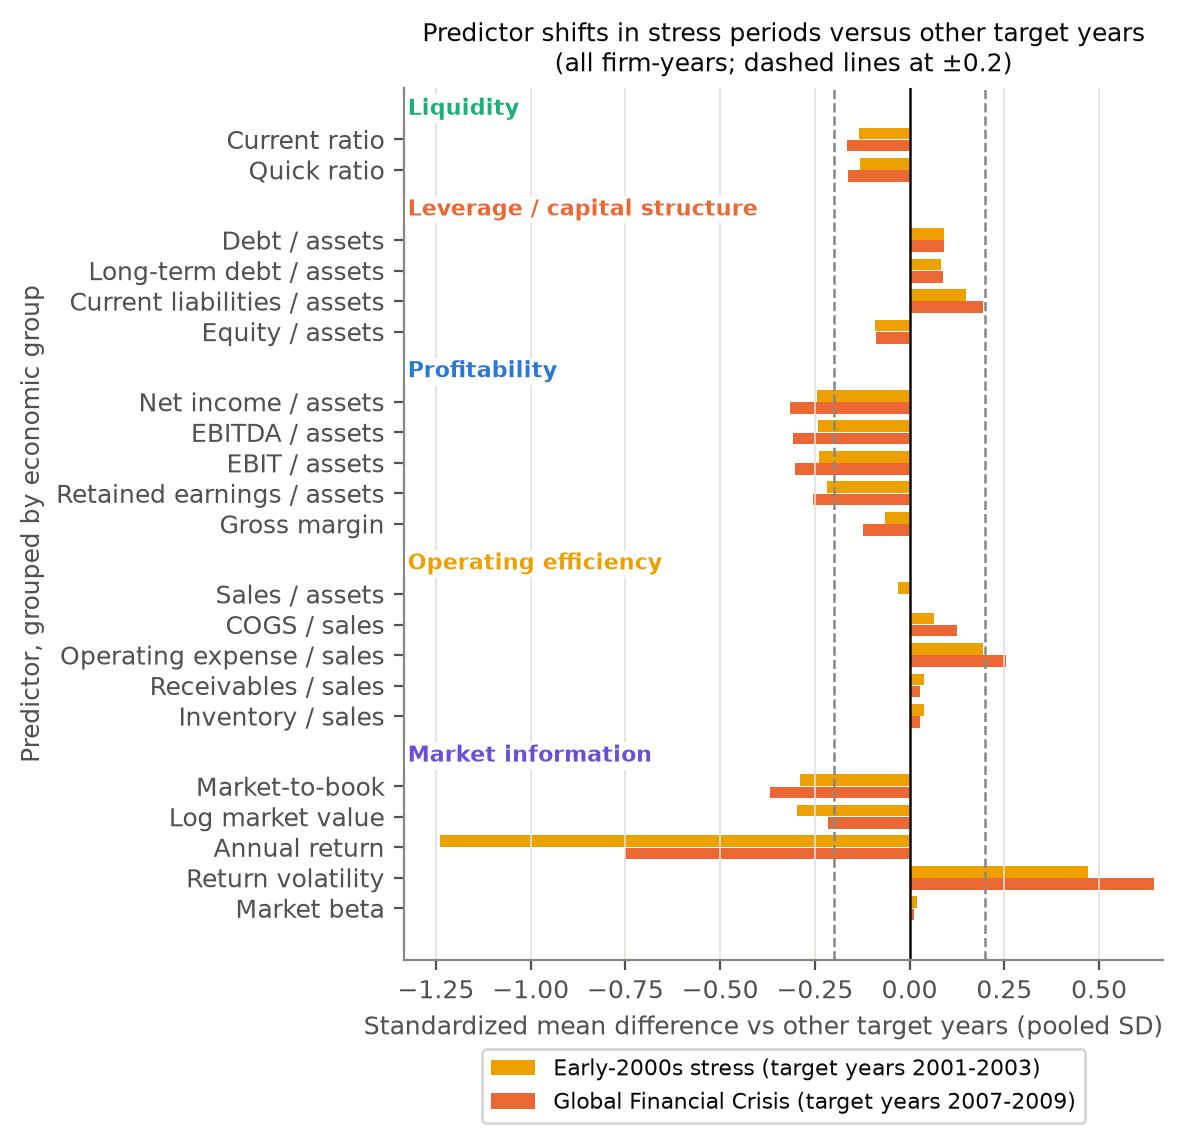
\includegraphics[width=0.595\textwidth]{stress_smd.png}
\par\vspace{1pt}
\captionof{figure}{Standardized mean differences (pooled SD) of the 21 predictors: early-2000s (2001--2003) and crisis (2007--2009) against all other target years.}
\end{center}

\begin{itemize}
  \item \textbf{Default rates.} Periods are target years 2001--2003 and 2007--2009 (predictors from fiscal years 2000--2002 and 2006--2008), compared with all other target years and with the other training years. The early-2000s rate is 0.23\%, below the other years' 0.78\% (no default spike in this dataset); the crisis rate is 1.40\%, 1.79 times the other years. Both lie in training (in-sample).
  \item \textbf{Largest shifts (Figure 6).} Against all other target years, 8 and 9 of 21 predictors shift notably (absolute SMD at least 0.20) in the early-2000s and the crisis, but only 3 and 6 against the other training years, so differences between earlier and later years (time trends or changing sample mix) contribute. Shifts holding under both: Annual return, Return volatility and Market-to-book in both periods, profitability only in the crisis. Annual return is also first in Ridge and XGBoost permutation importance, but Return volatility ranks 9 and 15 and Market-to-book 20 and 20, so a large shift is not importance.
  \item \textbf{Accounting versus market information.} In the crisis the market-only model has ROC-AUC 0.620 against 0.711 for the accounting-only model ($-$0.091 [$-$0.133, $-$0.048], lower); other periods are similar. The accounting block has 14 predictors and the market block 5, both scored in-sample, so the larger block has a mechanical advantage; market information is not shown to help.
  \item \textbf{Signs to monitor.} Concrete in-sample result: the same fitted Ridge over-predicts the early-2000s years (mean 0.81\% against 0.23\% observed, interval 0.16\% to 0.32\%) and under-predicts the crisis years (0.87\% against 1.40\%, 1.21\% to 1.63\%), so the mapping from characteristics to default differs across these regimes (descriptive). The market-versus-accounting gap is detectable only in the crisis years, and test ROC-AUC exceeds validation ROC-AUC for every frozen model (different samples, intervals overlapping). Relationships can shift with credit conditions, policy support and market co-movement. Monitor rates and predictor averages by year (later firm-years look safer on return, volatility and size), recalibrate when they diverge, keep XGBoost as challenger.
\end{itemize}

\subsection*{Recommendation for a credit-risk team}
{\small
\begin{itemize}
  \item \textbf{Deploy Ridge, with XGBoost as challenger.} The rule fixed on validation before the test years applies: the best model by validation ROC-AUC is itself linear, Ridge (0.697 against 0.696 for LASSO), so the rule coincides with the highest validation ROC-AUC (the 0.0001 tie tolerance acts as a strict maximum). Test and stress results were not used; its test ROC-AUC (0.738) is higher than the tree and Model 1. Ridge and LASSO are similar on validation (LASSO minus Ridge $-$0.001 [$-$0.006, +0.005]) and test (+0.004 [$-$0.0002, +0.009], the interval only just including zero), so the data do not separate them: LASSO is an equally defensible, sparser choice (18 of 31 coefficients zeroed; 19 in an alternative solution with the same fit), Ridge keeps correlated groups with shrunken weights (a possible stability advantage, not tested here), and choosing LASSO for its higher test ROC-AUC (0.742) would use test outcomes. ``Not automatically'' also means not preferring complexity for a small, noisy margin: Ridge is similar to the forest and XGBoost on validation, higher than the tree.
  \item \textbf{Criteria.} Ranking: Ridge's top decile holds 38.7\% of test defaults. Calibration: apply the validation Platt map and refresh it. Interpretability: a transparent linear link with sensible signs (associations, not causal). Stability: the in-sample over- and under-prediction by regime above, raw Ridge test-year means 0.50\% to 0.62\% against observed 0.70\% to 1.32\% across test years, and the market-versus-accounting contrast appears only in the crisis years; none is established across regimes. False-positive costs: 187 false alarms against 16 detected defaults at the validation threshold (not cost-based): set the cut-off from the cost of a missed default versus a false alarm.
\end{itemize}
}

\subsection*{Limitations}
{\small
\begin{itemize}
  \item Anonymized teaching data on a synthetic scale (results illustrate methods, not real-world magnitudes); only 87 validation and 119 test defaults, four test fiscal years, one chronological split: small gaps can be noise and other periods could rank models differently; every validation and test firm also appears in training, so results describe later years of observed firms.
\end{itemize}
}

\end{document}
